\documentclass[a4paper, 12pt]{scrartcl}

\usepackage{a4wide}
\usepackage[utf8]{inputenc}
\usepackage[ngerman]{babel}
\usepackage[T1]{fontenc}
\usepackage{amsmath}
\usepackage{graphicx}
\usepackage{listings}
\usepackage{hyperref}
\usepackage{xcolor}

\usepackage{setspace}

%%%%%%%%%%%%%%%%%%%%%%%%%%%%%%%%%%%%%%%%%%%%%%%%%%%%%%%%%
%
% Listings
%
% TODO:
%  - aufräumen
%  - besser strukturieren
%
%%%%%%%%%%%%%%%%%%%%%%%%%%%%%%%%%%%%%%%%%%%%%%%%%%%%%%%%%

\definecolor{lightgray}{rgb}{0.95, 0.95, 0.95}
\definecolor{darkgray}{rgb}{0.4, 0.4, 0.4}
%\definecolor{purple}{rgb}{0.65, 0.12, 0.82}
\definecolor{editorGray}{rgb}{0.95, 0.95, 0.95}
\definecolor{editorOcher}{rgb}{1, 0.5, 0} % #FF7F00 -> rgb(239, 169, 0)
\definecolor{editorGreen}{rgb}{0, 0.5, 0} % #007C00 -> rgb(0, 124, 0)
\definecolor{green}{rgb}{0, 0.8, 0}
\definecolor{orange}{rgb}{1,0.45,0.13}
\definecolor{olive}{rgb}{0.17,0.59,0.20}
\definecolor{brown}{rgb}{0.69,0.31,0.31}
\definecolor{purple}{rgb}{0.38,0.18,0.81}
\definecolor{lightblue}{rgb}{0.1,0.57,0.7}
\definecolor{lightred}{rgb}{1,0.4,0.5}
\definecolor{darkblue}{rgb}{0.0,0.0,0.6}
\definecolor{cyan}{rgb}{0.0,0.6,0.6}


% Default style for listings
\lstset{
  backgroundcolor=\color{editorGray},
  basicstyle={\footnotesize\ttfamily},
  breakatwhitespace=true,
  breaklines=true,   % sets automatic line breaking
  captionpos=b,      % sets the caption-position to bottom
  keepspaces=true,   % keeps spaces in text, useful for keeping indentation
  					 % of code (possibly needs columns=flexible)
  showspaces=false,  % show spaces everywhere adding particular underscores;
  					 % it overrides 'showstringspaces'
  showstringspaces=false, % underline spaces within strings only
  showtabs=false,         % show tabs within strings adding particular underscores
  tabsize=2,	          % sets default tabsize to 2 spaces
  rulecolor=\color{darkgray},   % if not set, the frame-color may be changed on
  								% line-breaks within not-black text
  								% (e.g. comments (green here))
  %numberstyle=\tiny\color{black}, % the style that is used for the line-numbers
  frame=tb,
  % line-numbers
  numbersep=5pt,     % how far the line-numbers are from the code
  stepnumber=1,
  firstnumber=1,
  numberfirstline=true,
  %xleftmargin={0.75cm},
  numbers=left,      % where to put the line-numbers; possible
  					 % values are (none, left, right)
  identifierstyle=\color{black},
  keywordstyle=\color{blue},
  stringstyle=\color{editorOcher},
  commentstyle=\color{brown}
}

\usepackage{tikz}
\usetikzlibrary{positioning,calc,shapes,arrows,shapes.multipart}

\newcommand*{\quelle}{% 
  \footnotesize Quelle: 
} 


\usepackage{scrpage2}
\pagestyle{scrheadings}
\clearscrheadfoot

\makeatletter

\def \autorenWithMatr {Felix Starke (Matr.: )\\
 Lars Hübner (Matr.: 5485901)} % MATRIKELNUMMER
\def \autoren {Felix Starke, Lars Hübner}
\def \titel {Metronom für Intel 8051}
\def \arbeit {Projekt Systemnahe Programmierung}
\def \uni {DHBW Karlsruhe}
\def \betreuer {Prof. Dr. Ralph Lausen}
\def \datum {6. Juni 2018}

\title{\titel}
\author{\autorenWithMatr}
\date{\datum}

\ihead{\titel}
\ohead{\autoren}
\ofoot{\pagemark}

\begin{document}
\begin{onehalfspace}

\begin{titlepage}
	\centering
	
\includegraphics[width=0.4\textwidth]{dhbw.png}\par\vspace{1cm}
	{\scshape\LARGE \uni \par}
	\vspace{1cm}
	{\scshape\Large \arbeit\par}
	\vspace{1.5cm}
	{\huge\bfseries \titel\par}
	\vspace{2cm}
	{\Large\itshape \autorenWithMatr\par}
	\vfill
	betreut von\par
	\textsc{\betreuer}

	\vfill

% Bottom of the page
	{\large \datum\par}
\end{titlepage}

\newpage
\tableofcontents
\newpage

\section{Einleitung}
\subsection{Motivation}
Ein Metronom beschreibt ein mechanisches oder elektronisches Gerät, welches zur regelmäßigen Tonerzeugung genutzt wird um musikalische Rhythmen zu unterstützen. Die Mehrzahl der neueren Metronome haben eine Funktion, bei der über ein regelmäßiges Klicken auf einen Button der entsprechende Klick-Takt übernommen wird.
\\
Da Metronome häufig als kleine portable Geräte mit geringem Stromverbrauch umgesetzt werden, kann eine entsprechende Funktionalität auf einem Intel 8051 Mikrocontroller implementiert werden. Die Programmierung auf diesem Mikrocomputer geschieht in Assembler. Ziel dieses Projektes ist entsprechend die Implementierung einer solchen "Tap to Beat" Funktion in Assembler für den 8051.

\subsection{Aufgabenstellung}
Aus diesen Anforderungen ergibt sich die folgende Aufgabenstellung.
\\
Das Programm muss eine Funktionalität implementieren, die das Aufnehmen des Taktes über eine Eingabehardware ermöglicht. Außerdem muss das Ausgeben des Taktes über eine passende Ausgabehardware implementiert werden.
Das gesamte Programm lässt sich damit in zwei große Teile splitten, dass Recording und das Anzeigen des Taktes.
\\
\\
\textbf{Recording}
\\
Die Aufnahme des Taktes muss über eine Eingabehardware getätigt werden. In diesem Projekt wurde eine Keypad-Matrix mit Tasten als Eingabe gewählt. Über eine dieser Tasten soll nun der Takt gemessen werden. Hierzu wird jeweils die Zeitspanne zwischen zwei Tastendrücken mithilfe eines Timers gemessen. Die Messungen sollen im Anschluss auf summiert und am Ende durch die Anzahl der Messungen geteilt werden, um den Mittelwert zu erhalten.
\\
\\
\textbf{Display Metronom}
\\
Nachdem der durchschnittliche Takt gemessen und ermittelt wurde, gilt es diesen auf einem Ausgabemedium anzuzeigen. Anstelle einer Tonausgabe wird in dieser Implementierung eine LED-Matrix genutzt um den Takt zu visualisieren.
\newpage
\section{Grundlagen}
\subsection{Assembler}
Assembler ist eine maschinenorientierte Programmiersprache, welche auf einem prozessorspezifischen Befehlssatz basiert. Die Sprache wird als Programmiersprache der zweiten Generation bezeichnet, da es nicht mehr notwendig ist, die Befehle als Binärcode zu schreiben. Statt dessen ist es möglich tatsächliche Befehle in Textform, wie zum Beispiel $"$ADD Op1, Op2$"$ zu verwenden. Assembler wird anschließend mit einem Assemblierer in den tatsächlichen Maschinencode übersetzt, welchen dann vom Prozessor ausgeführt wird.

\subsection{Intel 8051 Mikrocontroller}
Der Intel 8051 Mikrocontroller ist einer der am weitesten verbreiteten Mikrocontroller. Der 8051 ist ein 8-bit Mikrocontroller und kommt in verschiedensten Gebieten zum Einsatz. Dazu gehören beispielsweise die Automobilindustrie oder Anwendungen in der Robotik oder Telekommunikation. Er verfügt unter anderem über 4 KB Programmspeicher, 128 Byte Datenspeicher und zwei 16-Bit Timern. Des Weiteren existieren noch Varianten des Prozessors, die über besondere Komponenten wie beispielsweise UART verfügen und den Mikrocontroller entsprechend noch leistungsfähiger machen.
\begin{figure}[h]
\centering
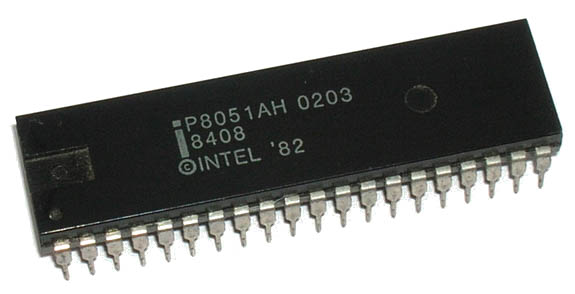
\includegraphics[width=0.7\textwidth]{8051.jpg}
\caption{Intel 8051}
\quelle\url{http://www.ne555.at/2014/images/stories/UC/Intel-P8051AH.jpg} 
\label{fig:mcu}
\end{figure}

\subsection{Entwicklungsumgebung MCU-8051}
Um eine einfachere und schnellere Entwicklung des Programmcodes zu ermöglichen wird zu Implementierung die MCU-8051 IDE verwendet. Diese IDE ermöglicht eine Virtualisierung der Hardware (des Intel 8051) sowie passende virtuelle Zusatzhardware für Eingaben und Ausgaben. \autoref{fig:mcu} zeigt die Entwicklungsumgebung.
\begin{figure}[h]
\centering
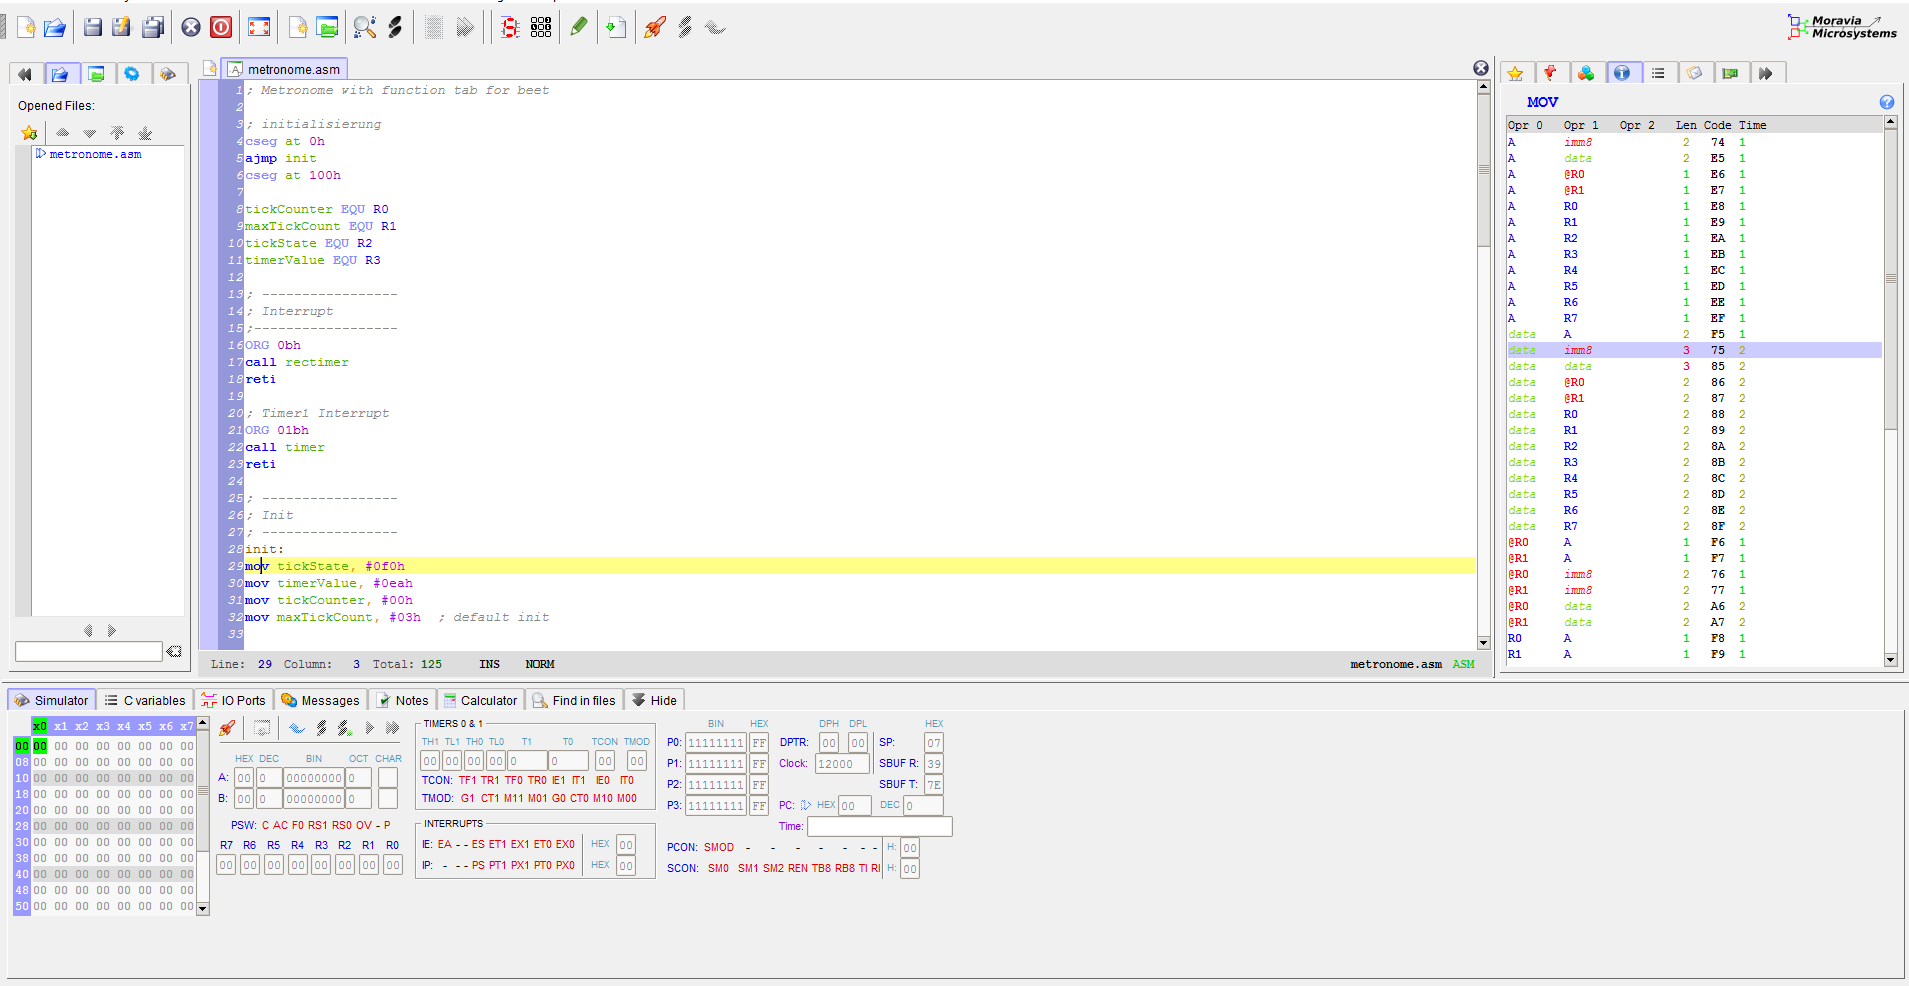
\includegraphics[width=\textwidth]{mcu.png}
\caption{MCU 8051 - IDE}
\label{fig:mcu}
\end{figure}

\newpage
\section{Konzept}
\subsection{Eingaben, Ausgaben und Ports}
Um dem Metronom den Takt vorzugeben, kommt eine 4x4 Keypad-Matrix (siehe \autoref{fig:keypad}) zur Eingabe zum Einsatz. Diese ist an alle acht Pins von Port 0 angeschlossen. Dabei werden die Pins 0-3 für die vier Spalten der Matrix und Pins 4-7 für die Zeilen der Matrix verwendet. Um eine gedrückte Teste zu detektieren müssen zunächst die Pins 0-3 auf "1" gesetzt werden und die Pins 4-7 gelesen werden. So lässt sich herausfinden, ob überhaupt eine Taste gedrückt ist und welcher Spalte diese angehört. Im nächsten Takt können dann die Pins 4-7 auf "1" gesetzt werden und 0-3 auf "0". Anschließend kann die Zeile der gedrückten Taste ermittelt werden.
\begin{figure}[h]
\centering
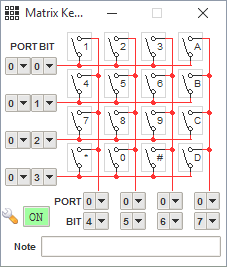
\includegraphics[width=0.5\textwidth]{keypad.png}
\caption{Keypad Matrix}
\label{fig:keypad}
\end{figure}
\\
\\
Für die Ausgabe des ermittelten Taktes wird eine 8x8 LED-Matrix (siehe \autoref{fig:led}) verwendet. diese ist an die Ports 2 und 3 angeschlossen. Die acht Pins von Port 2 werden genutzt um die Spalten der Matrix anzusteuern, die acht Pins von Port 3 werden für die Zeilen der LED-Matrix verwendet. Eine der 64 LED's leuchtet genau dann, wenn sowohl der Pin der entsprechenden Zeile als auch der entsprechenden Spalte gesetzt sind.
\begin{figure}[h]
\centering
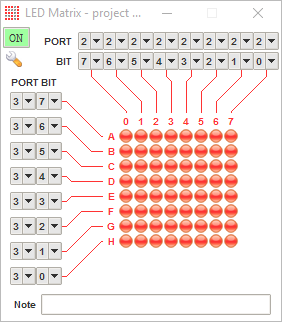
\includegraphics[width=0.5\textwidth]{led.png}
\caption{LED Matrix}
\label{fig:led}
\end{figure}
\subsection{Programmablauf}
Das Programm besteht wie beschrieben aus zwei Teilen. Im ersten Schritt wird zunächst der Takt ermittelt um diesen dann im zweiten Teil des Programms zu visualisieren.
\\
\\
Programmteil 1 besteht damit aus einer Schleife, die solange Zeitmessungen durchführt bis 3 Messungen vorhanden sind. Diese Schleife startet mit dem ersten Tastendruck auf das Keypad. Eine Messung ermittelt die Zeitspanne zwischen zwei Tastendrücken. 
\\
Nach dem genug Messungen durchgeführt wurden, kann die Summe der Zeitspannen durch die Anzahl (hier 3) geteilt werden, um so den mittleren Takt zu ermitteln. Diese Mittelwertrechnung ist deshalb wichtig, da der Mensch seinen Takt beim Drücken der Taste nicht konstant halten kann und so geringen Ungenauigkeiten entstehen.
\\
Durch die Mittelwertberechnung kann der Takt einfach gemittelt werden, um möglichst nah an den tatsächlichen Takt ran zu kommen. In \autoref{fig:pgmAblauf} ist der Programmablauf aus Programmteil 1 gezeigt.
% Include flow chart definition
% Define block styles
\tikzset{
   papDecision/.style = {
         diamond,
         draw, 
         text width = 20 mm, 
         align = center, 
         text badly centered,
         inner sep = 1 pt,
         font=\ttfamily\footnotesize,
         %line width = 1,
         minimum width = 30mm,
         minimum height = 7mm,
      },
   papStart/.style = {
         rectangle,
         draw, 
         align = center, 
         text width = 3cm, 
         text badly centered,
         inner sep = 4 pt,
         rounded corners=10pt,
         font=\ttfamily\footnotesize,
         %line width = 1,
         minimum width = 30mm,
         minimum height = 7mm,
      },
   papEnd/.style = {
         rectangle,
         draw, 
         align = center, 
         text width = 3cm, 
         text badly centered,
         inner sep = 4 pt,
         rounded corners=10pt,
         font=\ttfamily\footnotesize,
         %line width = 1,
         minimum width = 30mm,
         minimum height = 7mm,
      },
   papData/.style = {
         trapezium,
         draw, 
         align = center, 
         text width = 20 mm, 
         text badly centered,
         inner sep = 4 pt,
         trapezium left angle=70,
         trapezium right angle=110,
         font=\ttfamily\footnotesize,
         %line width = 1,
         minimum width = 30mm,
         minimum height = 7mm,
      },
   papPredProc/.style = {
         draw,
         rectangle split,
         rectangle split horizontal,
         rectangle split parts = 3,
         rectangle split empty part width=-8pt,
         align = center, 
 %       text width = 4.5 em, 
         text badly centered,
 %        inner sep = 4 pt,
         font=\ttfamily\footnotesize,
         %line width = 1,
         minimum width = 30mm,
         minimum height = 7mm,
      },
   papProcess/.style = {
         rectangle,
         draw,
         align = center, 
         text width = 3cm, 
         text badly centered,
         %inner sep = 2 pt,
         font=\ttfamily\footnotesize,
         %line width = 1,
         minimum width = 30mm,
         minimum height = 7mm,
      },
   papLine/.style = {
         draw,
         -stealth,
         font=\ttfamily\footnotesize,
         %line width = 1,
      },
}

\newcommand{\papYes}{ja}
\newcommand{\papNo}{nein}


%%%%%%%%%%%%%%%%%%%%%%%%%%%%%%%%%%%%%%%%%%%%%%%%%%%%%%%%%%%%%%%%%


\begin{figure}
\centering
\begin{tikzpicture}[node distance = 2cm, auto]

% Place nodes
\node [papStart] (Start1){Start};
\node [papProcess, below of = Start1] (pro1){Warte auf button};
\node [papDecision, below of = pro1, yshift= -9mm](dec1){Button gedrückt?};
\node [papProcess, below of = dec1] (pro2){Starte Timer};
\node [papProcess, below of = pro2] (pro3){Warte auf button};
\node [papDecision, below of = pro3, yshift= -9mm](dec2){Button losgelassen?};
\node [papProcess, below of = dec2] (pro4){Stope Timer};
\node [papProcess, below of = pro4] (pro5){Summiere Timer auf};
\node [papDecision, below of = pro5, yshift= -9mm](dec3){Button 3x gedrückt?};
\node [papProcess, below of = dec3] (pro6){Dividiere Summe durch 3};
\node [papEnd, below of = pro6] (End) {Starte Metronom};


% Draw edges
\path [papLine] (Start1) -- (pro1);
\path [papLine] (pro1) -- (dec1);
\path [papLine] (dec1.east) -| node [right] {\papNo}(2, -2) -- (pro1.east);
\path [papLine] (dec1) -- node [right] {\papYes} (pro2);
\path [papLine] (pro2) -- (pro3);
\path [papLine] (pro3) -- (dec2);
\path [papLine] (dec2.east) -| node [right] {\papNo}(2, -8.9) -- (pro3.east);
\path [papLine] (dec2) -- node [right] {\papYes} (pro4);
\path [papLine] (pro4) -- (pro5);
\path [papLine] (pro5) -- (dec3);
\path [papLine] (dec3.east) -| node [right] {\papNo}(4, -2) -- (pro1.east);
\path [papLine] (dec3) -- node [right] {\papYes} (pro6);
\path [papLine] (pro6) -- (End);

\end{tikzpicture}
\caption{Programmablauf} \label{fig:pgmAblauf}
\end{figure}
In Programmteil 2 kann der ermittelte Durchschnittswert genutzt werden, um den Takt mit Hilfe eines Timers auf der LED-Matrix zu visualisieren. Zur Visualisierung blinkt abwechselnd die linke und die rechte Hälfte der LED-Matrix auf. Dieses hin und her wechseln der Seiten erinnert somit an ein gewöhnliches Metronom. Hierbei ist zu vermerken, dass die Routine zum Zeichnen auf der LED-Matrix stark vereinfacht wurde, um den Geschwindigkeitsanforderungen gerecht zu werden und das Metronom trotz Simulation und virtueller Hardware nutzbar zu machen. In \autoref{schwierigkeiten} wird beschrieben, warum diese Schwierigkeit vorliegt und wie damit umgegangen wird.
\\  
Der Timerüberlauf wird zur Takterzeugung auf den in Teil 1 verwendeten Timerüberlauf gesetzt. Mit jedem Überlauf des Timers wird ein entsprechender Interrupt geworfen, welcher von einer Interruptrutiene (siehe timer function im asm-code) gefangen wird und eine passende visuelle Änderung auf der LED-Matrix veranlasst.
\\
\\
Wie in \autoref{lst:timer} gezeigt wird eine Art Bitmap eingeführt, welche als Indikator dafür dient, welche Spalten aufleuchten sollen. P2 (Port 2) ist mit der LED-Matrix verbinden und sorgt für die Ausgabe. Anschließend muss geprüft werden, ob bereits die in Teil 1 ermittelte Zeitspanne (in Anzahl Überläufen) abgelaufen ist. Um dies zu ermitteln wird der aktuelle tickCounter vom maxTickCounter (in Teil 1 ermittelt) abgezogen. Sobald des Ergebnis "0" erreicht muss der Zähler zurückgesetzt werden.
\\
Beim Zurücksetzen wird zusätzlich mit "cpl A" die Bitmap zur Visualisierung bitweise invertiert um so die leuchtende Seite der LED-Matrix zu ändern.

\begin{figure}
\begin{lstlisting}
timer:
mov P2, tickState	
inc tickCounter		

clr c
mov A, maxTickCount
subb A, tickCounter	
jnz keep
call resetTickCounter	
keep:
ret

resetTickCounter:
mov tickCounter, #00h	
mov A, tickState	
cpl A
mov tickState, A
ret
\end{lstlisting}
\caption{Interruptroutine}
\label{lst:timer}
\end{figure}

\newpage
\section{Besondere Schwierigkeiten}
\label{schwierigkeiten}
Besondere Schwierigkeiten ergaben sich aufgrund der hohen Laufzeiten durch die Entwicklungsumgebung. Vorallem die Nutzung virtueller Hardware verlangsamt den Ablauf des Programms stark. So vergehen, auf einem recht leistungsstarken Rechner, etwa 7 Sekunden, bis im Simulator der Entwicklungsumgebung eine Millisekunde verstrichen ist. Da gutes Timing für ein Metronom sehr wichtig ist, musste entschieden werden, wie mit der langsamen Laufzeit umgegangen werden sollte. Da das Metronom nutzbar sein sollte wurde das Timing nicht an der simulierten Laufzeit der Entwicklungsumgebung orientiert. Da weder die Eingabe zur Festlegung des Taktes noch die Ausgabe des Takts über die LED-Matrix an die Zeit der Simulation gebunden sind, ist es einfach möglich, beides zu synchronisieren und so umzusetzten, dass das Metronom nutzbar ist.

\newpage
\section{Zusammenfassung}
Das Metronom konnte vollständig funktionsfähig umgesetzt werden und erfüllt damit unsere Aufgabenstellung. Die Umsetzung dieses Projektes war eine ideale Möglichkeit, die Vorlesungsinhalte in der Praxis anzuwenden und zu vertiefen. So konnte der Umgang mit Mikrocontrollern und der Assemblerprogrammierung gelernt und damit verbundene Schwierigkeiten erfahren werden. Der Einsatz der Entwicklungsumgebung mit Simulation bringt zwar ebenfalls Herausforderungen mit sich, ist aber dennoch eine sehr gute Wahl, da so schwerwiegendere Probleme, die bei der Verwendung von echter Hardware auftreten können, vermieden werden können.

\newpage
\section*{Eidesstattliche Versicherung}
Wir versicheren hiermit, dass wir unser {\arbeit} mit dem Thema: {\itshape \titel } selbstständig verfasst und keine anderen als die angegebenen Quellen und Hilfsmittel benutzt haben. Wir versicheren zudem, dass die eingereichte elektronische Fassung mit der gedruckten Fassung übereinstimmt. 
\\
\\
\\
\\
\vspace{3em}
Karlsruhe, 29. Juni 2018
\vspace{4em}
\\
\rule{10cm}{0.4pt}\\
\autoren

\end{onehalfspace}
\end{document}
